\section{Referee} \label{sec:referee}

%Justification
\subsection{Justification} \label{referee-justification}
Once we had defined the datapath of the core, we were ready to expand our single-core design into a multi-core.
We can duplicate the datapath to generate as many cores as we desire. However, we will need to implement a shared memory design if we want them to communicate with each other through memory. 

Nevertheless, we cannot just create a single memory and connect all the cores to it. 
The original \textit{Darkriscv} design assumed an instantaneous memory that could complete read and write operations without delay, but we now have $N$ cores accessing the memory, so some will need to wait in the case of simultaneous accesses since we plan to serialize them.


%Behaviour
\subsection{Behaviour} \label{referee-behaviour}
We created a module calLED \textit{Referee}, which works as an interface between $N$ cores and the memory.
Its purpose is to grant access from the cores to the memory, halting the cores that must wait their turn to access it.
In a way, it acts as a single core from the memory side, so the memory is agnostic of the actual number of cores.
A simplified diagram of this module can be seen in Figure~\ref{referee-fig}.

\begin{figure}[h!]
    \centering
    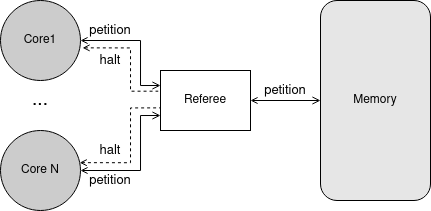
\includegraphics[width=.5\textwidth]{images/Referee_fig.png}
    \caption{Simplified diagram of the Referee.}
    \label{referee-fig}
\end{figure}

The \textit{Referee} treats read and write operations the same way.
For simplicity, we will refer to a \textit{petition} when we want to address both read and write operations.
If many cores send a petition at the same time, the \textit{Referee} chooses the one from the core with the highest ID, halts all the requesting cores, sends the petition to the memory, and waits for its answer.
If more cores try to access memory while an old petition is being served, the \textit{Referee} halts them.
When the memory finishes serving the petition, the core releases (unhalts) its associated core and serves the next petition.

%Verification
\subsection{Verification}
Once the module was designed, the next step was to test if it was working correctly.
In order to generate codes, we first write them with either assembly inline or C.
After that, we compile it with a modified \textit{gcc} supporting RISC-V found in the RISC-V Tools~\cite{tools} and then we use \textit{Objdump} to obtain the hexadecimal codification of the instructions.
This process is exemplified in Figure~\ref{coding}.

\begin{figure}[h!]
    \centering
    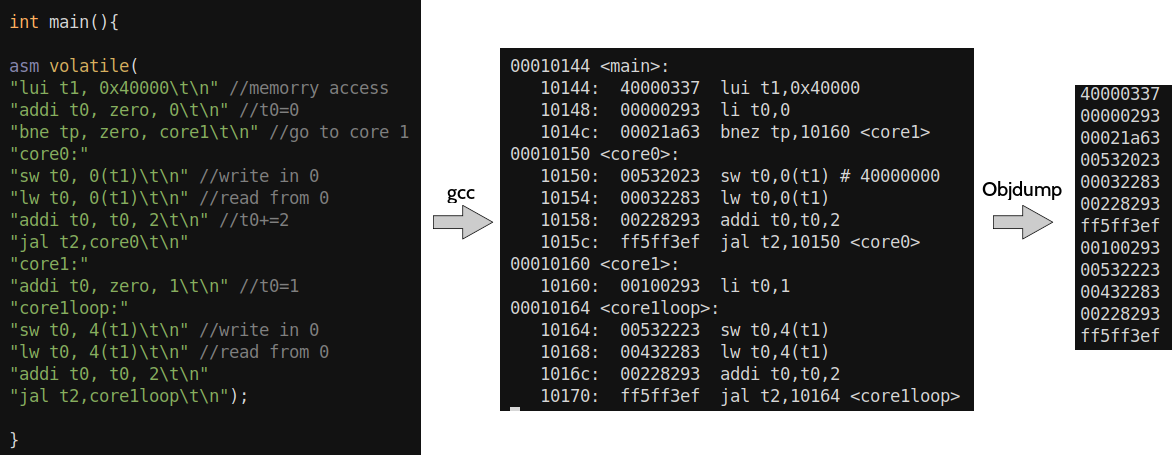
\includegraphics[width=.9\textwidth]{images/coding.png}
    \caption{Generating codes for Darkriscv.}
    \label{coding}
\end{figure}

Finally, the hexadecimal instructions are written in a file that acts as a ROM, embedded in the \gls{fpga} when generating the bitstream, or simply read when simulating.

The first test was to set the number of cores to 2 and run a straightforward code where they light up LEDs alternatively.



\begin{figure}[htbp]
\centering
\begin{minipage}[t][4cm][t]{4.5cm}
\textbf{Core 0}\\
while(1)\{\\
\hspace*{1cm}LEDs = [0 0 0 1];\\
\hspace*{1cm}flag0 = 1;\\
\hspace*{1cm}while(!flag1);\\
\hspace*{1cm}flag1 = 0;\\
\hspace*{1cm}LEDs = [0 1 0 0];\\
\}
\end{minipage}\hspace{2.5cm}
\begin{minipage}[t][4cm][t]{4.5cm}
\textbf{Core 1}\\
while(1)\{\\
\hspace*{1cm}while(!flag0);\\
\hspace*{1cm}flag0 = 0;\\
\hspace*{1cm}LEDs = [0 0 1 0];\\
\hspace*{1cm}flag1 = 1;\\
\}
\end{minipage}%
\vspace{.1cm}
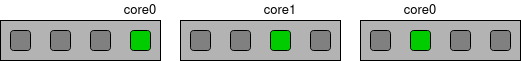
\includegraphics[width=.75\textwidth]{images/leds2_fig.png}
\caption{Pseudocode of the test code with 2 processors.}
\label{2LED-code}
\end{figure}
\clearpage
In Figure~\ref{2LED-code} we can find the pseudocode that both cores are running and a scheme of the expected behaviour.
Core 0 lights up the first LED, signals core 1 to light up the second one and then to signal core 0 again to light up the third LED.

Figure~\ref{2LED-sim} shows the simulation of this code.
We see how core 0 lights up the first LED and waits some cycles before setting flag0 to 1, while core 1 repeatedly reads the value of this flag.
Then, the same happens, changing the roles of core 0 and core 1.

\begin{figure}[h!]
    \centering
    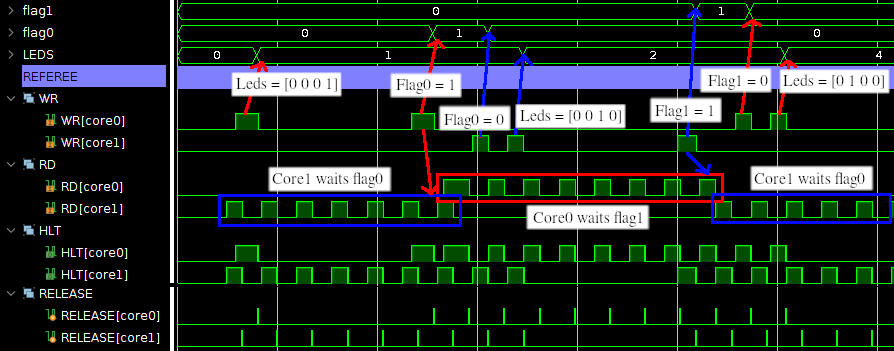
\includegraphics[width=1.0\textwidth]{images/flag2_sim_crop_arrows.png}
    \caption{Simulation of the code depicted in Figure~\ref{2LED-code}.}
    \label{2LED-sim}
\end{figure}


We can also zoom in to see an example of how the \textit{Referee} is working in this example. In Figure~\ref{2LED-close} we can see how core 0 tries to write while core 1 is waiting for the memory to complete a read petition.
The \textit{Referee} halts core 0 and does not send his petition until the read is finished.

\begin{figure}[h!]
    \centering
    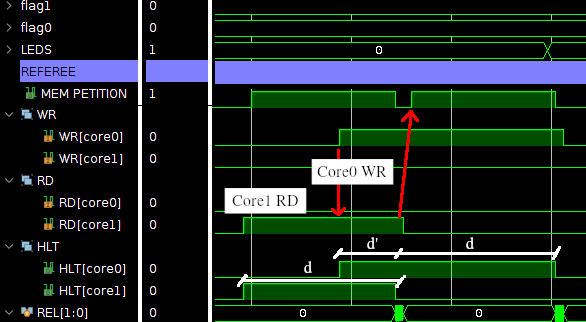
\includegraphics[width=0.7\textwidth]{images/flag2_sim_close_arrow.png}
    \caption{Simulation showing the serialitzation of memory accesses by the referee.}
    \label{2LED-close}
\end{figure}

Once we checked that this simple code was also working in the \gls{fpga}, we tried to complicate the design a little bit more.
We increased the number of cores from 2 to 4 and ran a very similar code, depicted in Figure~\ref{4LED-code}.
Core $i$ lights up LED $i$ and signals core $i+1$ to the same.

\begin{figure}[htbp]
\centering
\begin{minipage}[t][3cm][t]{3.2cm}
\textbf{Core 0}\\
while(1)\{\\
\hspace*{.4cm}while(flag!=0);\\
\hspace*{.4cm}LEDs=[0 0 0 1];\\
\hspace*{.4cm}flag=1;\\
\}
\end{minipage}\hspace{.5cm}
\begin{minipage}[t][3cm][t]{3.2cm}
\textbf{Core 1}\\
while(1)\{\\
\hspace*{.4cm}while(flag!=1);\\
\hspace*{.4cm}LEDs=[0 0 1 0];\\
\hspace*{.4cm}flag=2;\\
\}
\end{minipage}\hspace{.5cm}
\begin{minipage}[t][3cm][t]{3.2cm}
\textbf{Core 2}\\
while(1)\{\\
\hspace*{.4cm}while(flag!=2);\\
\hspace*{.4cm}LEDs=[0 1 0 0];\\
\hspace*{.4cm}flag=4;\\
\}
\end{minipage}\hspace{.5cm}
\begin{minipage}[t][3cm][t]{3.2cm}
\textbf{Core 3}\\
while(1)\{\\
\hspace*{.4cm}while(flag!=4);\\
\hspace*{.4cm}LEDs=[1 0 0 0];\\
\hspace*{.4cm}flag=0;\\
\}
\end{minipage}
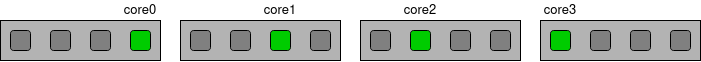
\includegraphics[width=.72\textwidth]{images/leds4_fig.png}
\caption{Pseudocode of the test code with 4 processors.}
\label{4LED-code}
\end{figure}

We simulated the code and found that it got stuck in an infinite deadlock.
In Figure~\ref{4LED-sim-bad} we can see how core 0 never gets his petition served.
Since core 0 is the first core to signal the next cores to do their work, they will keep reading the value of a flag that will never change.

\begin{figure}[h!]
    \centering
    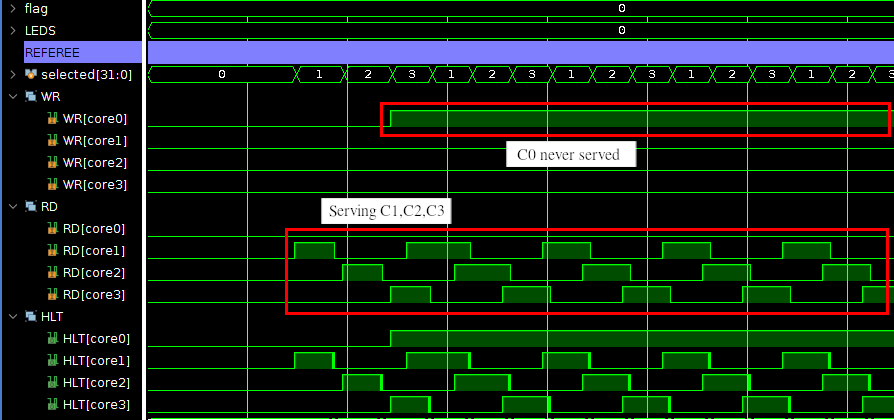
\includegraphics[width=1.0\textwidth]{images/flag4_sim_bad_crop_arrow.png}
    \caption{Simulation showing the memory hog problem.}
    \label{4LED-sim-bad}
\end{figure}

In Section~\ref{referee-behaviour} we mentioned that the \textit{Referee} prioritizes the core with the highest ID, if multiple were trying to access memory.
This explains what we see in Figure~\ref{4LED-sim-bad}.
At any point where the petition from core 0 is considered, a petition from a higher ID core is also active, so it does not get a chance to access memory.

To solve this, we changed how the served core is selected.
The \textit{Referee} has a register holding the prioritized core to serve.
It will always serve that core first if it is among the requesting cores when it receives multiple petitions.
If this is not the case, it selects the highest ID core from the rest.
After any petition, the register holding the prioritized core is increased.
This method ensures that all cores will get a chance to access memory, with a wait time of at most $N-1$ petitions in the worst case (i.e., when the core tries to access memory just after its turn has passed).

%figure showing this behavior?

After implementing this new logic, we simulated the same code from Figure~\ref{4LED-code} again and saw that everything was working as expected and the LEDs followed the desired pattern.

Finally, we tested a more realistic code.
We selected the \textit{dot product}, since it is really easily parallelized.
Remember that given two vector $v$ and $u$ of $n$ elements, the dot product is defined as $\sum_{i=0}^{n}{v_{i} * u_{i}}$.

In this case, we coded in C instead of in assembly to test how our design behaves when we do not manually pick the instructions but instead use a compiler.
The code follows these steps:
\begin{enumerate}
	\item Core 0 initializes the vectors to known values.
	\item All cores synchronize in a barrier.
	\item Every core computes its part of the sum ($\frac{n}{Ncores}$).
	\item In a reduction, each core accumulates its result in the same memory position.
\end{enumerate}

While most of the code can be done with plain C, we had to do some tweaks.
At the program's start, the stack pointer is manually set to an arbitrary position for each core, directly modifying the $sp$ register.
This is exemplified in Figure~\ref{stackfig}.

\begin{figure}[h!]
    \centering
    \begin{lstlisting}
asm volatile(
	"lui sp, 0x80000\t\n" //set up base stack
	"slli t0, tp, 7\t\n" //t0 = coreID*128
	"add sp, sp, t0\t\n" //sp = sp + t0;
);
    \end{lstlisting}
%    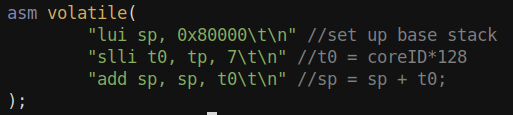
\includegraphics[width=.6\textwidth]{images/stack_ini.png}
    \caption{Initialization of the stack for multiple cores.}
    \label{stackfig}
\end{figure}

Furthermore, the global variables used to hold the vectors, synchronization flags, counters, and the final result are all pointers to an arbitrary position starting at 0x40000000, which is the start of the memory region to put the data.

The most interesting parts of the code are the barrier and the reduction, which work similarly.
In Figure~\ref{barrier} we show the code used for the barrier.

\begin{figure}[h!]
    \centering
    %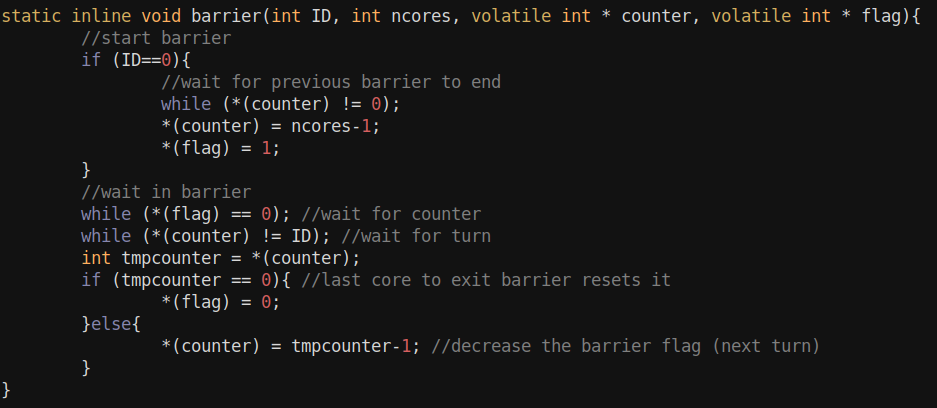
\includegraphics[width=.9\textwidth]{images/barrier.png}
    \begin{lstlisting}
static inline void barrier(int ID, int ncores, volatile int * counter, volatile int * flag){
	//start barrier
	if (ID==0){
		//wait for previous barrier to end
		while (*(counter) != 0);
		*(counter) = ncores-1;
		*(flag) = 1;
	}
	//wait in barrier
	while (*(flag) == 0); //wait for counter
	while (*(counter) != ID); //wait for turn
	int tmpcounter = *(counter);
	if (tmpcounter==0){//last core to exit barrier resets it
		*(flag) = 0;
	}else{
		*(counter) = tmpcounter-1; //decrease the barrier flag (next turn)
	}
}
    \end{lstlisting}
    \caption{Code snippet of the implemented barrier.}
    \label{barrier}
\end{figure}

Both are formed with a flag and a counter, which are both initialized at 0.
When core 0 arrives to the barrier, it sets the flag to 1 and sets the counter to $Ncores - 1$.
All cores except core 0 will wait until the flag is set and the counter equals their ID.
When that happens, they decrement the counter so the next core can do the same.
Then, the last core to exit the barrier resets it for future use.


The reduction works exactly the same, but with each core updating the content of the reduction variable when it is their turn.
It is important to note that in order for this code to work, each core has two registers hardcoded to its core ID and the total number of cores.


In Figure~\ref{4dot-sim} we see the simulation of the dot product with 4 cores.
We can see how core 0 initializes the vectors while the rest wait in the barrier until its flag is set to 1 and the counter decreases to 0.
Then, all cores compute their work, accessing their part of the vectors, and wait until core 0 starts the reduction.
Here, the same behavior as in the barrier is found until the correct result of 14 is generated.


\begin{figure}[h!]
    \centering
    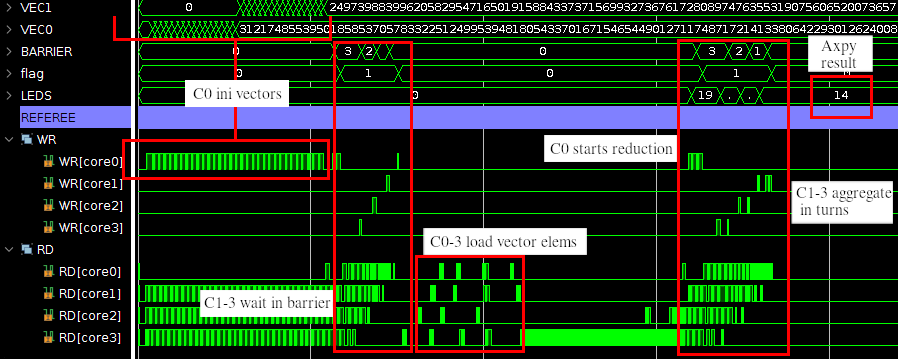
\includegraphics[width=1\textwidth]{images/axpy_sim4_crop_arrow.png}
    \caption{Simulation of the dot product with 4 cores.}
    \label{4dot-sim}
\end{figure}

We have also simulated it with 8 cores to show that the code is Ncores-agnostic, as can be seen in Figure~\ref{8dot-sim}.
The barrier and the reduction are longer, but the same result is obtained.

\begin{figure}[h!]
    \centering
    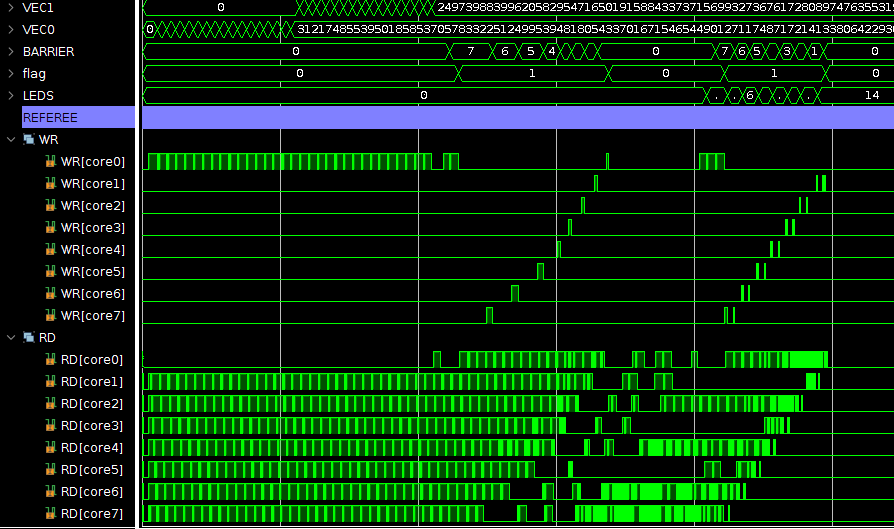
\includegraphics[width=.9\textwidth]{images/axpy_sim8_crop.png}
    \caption{Simulation of the dot product with 8 cores.}
    \label{8dot-sim}
\end{figure}










